\chapter{Учебные примеры}
В этой главе мы опишем подробно процесс установки, моделирования и пост- процесорной обработки для некоторых тестовых
 примеров OpenFOAM, с основной целью: познакомить пользователя с основными процедурами работы и управления OpenFOAM.
 \textit{\$FOAM\_TUTORIALS} директория содержит много тестовых случаев, которые демонстрируют использование всех
 решателей и многих утилит поставляемых с OpenFOAM. Прежде чем пытаться использовать обучающие программы, пользователь
 должен предварительно удостовериться  в том, что он установил OpenFOAM правильно.

Обучающие примеры описывают использование утилиты \textsl{blockMesh} - инструмента предпроцессорной обработки, установки 
примера и запуска на счет решателя OpenFOAM и постпроцессорной обработки с использованием \textsl{paraFoam}.
 Те пользователи, которые имеют доступ к постпроцессорам, разработанным другими фирмами (из инструментария посторонних
 разработчиков), также поддерживаемых в OpenFOAM, имеют выбор: либо они могут следовать за примерами обучающих программ,
 используя \textsl{paraFoam}; либо обратиться к описанию использования продукта постороннего разработчика, как описано в
главе 6, когда требуется постпроцессорная обработка.

Копии всех обучающих программ доступны в директории \textit{tutorials} из поставки OpenFOAM.
Обучающие программы организованы
 в виде ряда директорий согласно типу течения в которых расположены поддиректории согласно решателю. Например,
 все \textsl{icoFoam} примеры хранятся в пределах подкаталога \textit{incompressible/icoFoam}, где \textit{incompressible}
(несжимаемое)  указывает на тип рассматривваемого течения. Если пользователь желает запустить на расчет несколькотестовых 
примеров,  рекомендуется, чтобы пользователь сначала скопировал директорию \textit{tutorials} в свою локальноую директорию
\textit{run}. Они могут быть легко скопированы набором:

\texttt{mkdir –p \$FOAM\_RUN}

\texttt{cp –r \$FOAM\_TUTORIALS \$FOAM\_RUN}

\section{Течение в прямоугольной полости, инициированное верхней плитой}
\label{sec:2.1}
Этот раздел руководства описывает как выполнить этапы пре-процессор, расчет и постпроцессорную обработку для тестового
 примера, рассматривающего изотермическое течение несжимаемой среды в двумерной квадратной области. Геометрия течения
изображена на Рис. 2.1, в которой все границы квадрата являются стенками. Верхняя стенка перемещается в
\textit{x}-направлении со скоростью 1 м/с, в то время как другие 3 неподвижны. Первоначально принято, что будет
 рассматриваться ламинарное течение и задача будет решаться на однородной сетке, используя решатель \textsl{icoFoam}
 для ламинарного, изотермического, несжимаемого потока. В течение курса обучающей программы, будут исследованы влияние
 увеличения числа узлов сетки на решение и влияние измельчения шага сетки по направлению к стенкам.
Наконец, число Рейнольдса будет увеличено, и решатель \textsl{pisoFoam} будет использоваться для турбулентного,
 изотермического, несжимаемого течения.

\begin{figure}[h]
 \centering
 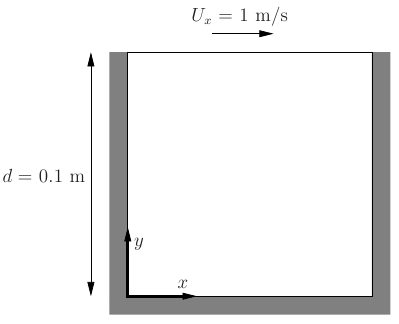
\includegraphics[width=299pt,height=243pt]{UGFigure2-1.PNG}
 % UGFigure2-1.PNG: 399x324 pixel, 96dpi, 10.56x8.57 cm, bb=0 0 299 243
 \caption{Геометрия течения в каверне, инициированного движением верхней плиты.}
 \label{fig:2.1}
\end{figure}

\section{Пре- процессорная подготовка (pre-processing)}
\label{sec:2.1.1}

В составе дистрибутива OpenFOAM поставляются примеры. Для редактирования файлов примера пользователь должен выбрать
 xeditor или другой редактор , типа \textbf{emacs}, \textbf{vi}, \textbf{gedit}, \textbf{kate}, \textbf{nedit},
 и т.п. Редактирование файлов возможно в OpenFOAM, потому что ввод / вывод использует формат словаря с ключевыми
 словами, которые представляют смысловое значение, чтобы быть понятными даже наименее опытным пользователям.

Моделируемый случай включает данные для сетки, полей, свойств, параметров контроля решения, и т.д.
 Как описано в секции 4.1, в OpenFOAM эти данные хранятся в ряде файлов в пределах директории примера,
 а не в единственном файле примера, как во многих других пакетах вычислительной гидродинамики (CFD).
 Директории примера дают соответственно описательное название, например первый случай для этого
 обучающего примера просто назван \textsl{cavity} (каверна). В подготовке редактирования файлов примера и
 запуска первого примера \textsl{cavity}, пользователь должен перейти в каталог примера

\texttt{cd \$FOAM\_RUN/tutorials/incompressible/icoFoam/cavity}

\subsection{Генерация сетки}
\label{sec:2.1.1.1}

OpenFOAM всегда работает в 3 мерной декартовой системе координат и все геометрические конфигурации производятся
 в 3 измерениях. OpenFOAM решает примеры в 3 измерениях по умолчанию, но может быть проинструктирован решать
 в 2 измерениях, определяя специальное \textsl{empty} (пустое) граничное условие на границах, нормальных к (3-ему)
 z измерению (для данного примера), для которого никакое решение проводить не требуется.
Область примера \textsl{cavity} состоит из квадрата c длинами сторон \textit{d} = 0.1 м. в \textit{x-y} плоскости.
Первоначально будет использоваться равномерная сетка 20 на 20 ячеек. В блочной конструкции показанной на Рис. 2.2. генератор сеток,
 поставляемый с OpenFOAM, \textit{blockMesh}, создает сетки, используя команды из описания определенного в словаре ввода,
 \textit{blockMeshDict} расположенного в каталоге \textit{constant/polyMesh} данного примера. Чтобы перейти к
 \textit{blockMeshDict}  для этого примера  возьмем следующий файл:
\begin{verbatim}
/*--------------------------------*- C++ -*----------------------------------*\
| =========                 |                                                 |
| \\      /  F ield         | OpenFOAM: The Open Source CFD Toolbox           |
|  \\    /   O peration     | Version:  2.1.0                                 |
|   \\  /    A nd           | Web:      www.OpenFOAM.com                      |
|    \\/     M anipulation  |                                                 |
\*---------------------------------------------------------------------------*/
FoamFile
{
    version     2.0;
\end{verbatim} 

\begin{figure}[h]
 \centering
 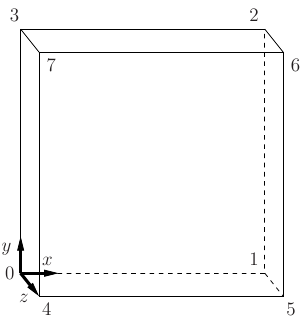
\includegraphics[width=229pt,height=241pt]{UGFigure2-2.PNG}
 % UGFigure2-2.PNG: 306x321 pixel, 96dpi, 8.10x8.49 cm, bb=0 0 229 241
 \caption{Блочная конструкция сетки для каверны.}
 \label{fig:2.2}
\end{figure}

\begin{verbatim}
    format      ascii;
    class       dictionary;
    object      blockMeshDict;
}
// * * * * * * * * * * * * * * * * * * * * * * * * * * * * * * * * * * * * * //

convertToMeters 0.1;

vertices        
(
    (0 0 0)
    (1 0 0)
    (1 1 0)
    (0 1 0)
    (0 0 0.1)
    (1 0 0.1)
    (1 1 0.1)
    (0 1 0.1)
);

blocks          
(
    hex (0 1 2 3 4 5 6 7) (20 20 1) simpleGrading (1 1 1)
);

edges           
(
);

boundary
(
    movingWall 
    {
        type wall;
        faces
        (
            (3 7 6 2)
        );
    }
    fixedWalls 
    {
        type wall;
        faces
        (
            (0 4 7 3)
            (2 6 5 1)
            (1 5 4 0)
        );
    }
    frontAndBack 
    {
        type empty;
        faces
        (
            (0 3 2 1)
            (4 5 6 7)
        );
    }
);

mergePatchPairs 
(
);

// ************************************************************************* //

\end{verbatim}

В начале файла содержится заголовок в форме баннера (строки 1-7), далее информация файла
 содержится в подсловаре \textsl{FoamFile}, заключенная в фигурных скобках ({...}).

\textit{В остальной части руководства:}
Ради сохранения места и для ясности, шапка или заголовок файла, включая баннер и \textsl{FoamFile} подсловарь,
 и обрамление в скобках не будут включаться в файлы примеров.

Файл в начале содержит блок вершин \texttt{vertices} (x,y,z координаты точек); затем в нем определяются сами блоки
 (\texttt{blocks})  (в данном примере имеется только 1) с помощью описанных выше меток вершин и номеров
 ячеек внутри них; и наконец, в файле определяются поверхности для задания граничных патчей.
 Пользователю предлагается обратиться к секции 5.3 чтобы понять значение вводимых  величин в \textsl{blockMeshDict} файле.

Сетка генерируется при запуске утилиты \textsl{blockMesh}, использующей файл \textsl{blockMeshDict}.
Запуск производится из директории задачи, просто набором команды в терминале:

\texttt{blockMesh}

Состояние выполнения \textsl{blockMesh} выводится в окне терминала. Любые ошибки в исходном 
файле сетки \textsl{blockMeshDict} обрабатываются textsl{blockMesh} и итоговые сообщения об ошибках показывают 
пользователю номер строки в которой возникла проблема. На этой стадии не должно быть никаких сообщений об ошибках.

\subsection{Граничные и начальные условия (условия однозначности)}
\label{sec:2.1.1.2}
